\documentclass[a4paper]{article}

\usepackage{fullpage} % Package to use full page
\usepackage{parskip} % Package to tweak paragraph skipping
\usepackage{tikz} % Package for drawing
\usepackage{amsmath}
\usepackage{hyperref}
\hypersetup{
    colorlinks=true,
    linkcolor=cyan,
    filecolor=magenta,      
    urlcolor=blue,
}
\usepackage{marginnote}

\newcommand{\argmaxF}{\mathop{\mathrm{argmax}}\limits}

\title{1: Introduction to RL\vspace{-2ex}}
\author{Ameya Godbole}
\date{\vspace{-5ex}}

\begin{document}

\maketitle

\section{Acknowledgement}

A thanks to:
\begin{enumerate}
\item the course instructor: Prof. Balaraman Ravindran (IIT Madras)
\item National Programme on Technology Enhanced Learning (NPTEL), India
\end{enumerate}

\section{Roots in behavioural psychology}
\textbf{Pavlov's dog}: Dog was contitioned to expect food after a bell. It formed the association resulting in it starting to salivate at the sound of a bell even when no food was given. Based on experiments in this vein, theories were formulated about how learning proceeds.

\section{What is reinforcement learning}
\begin{itemize}
\item Reinforcement learning is a mathematical formulation for a \textbf{trial-and-error} kind of learning.
\item It is a paradigm where we learn about a system through interaction.
\item Learning about stimuli and actions through \textbf{rewards and punishment alone}.
\item No detailed supervision is available. E.g. no one give a value of force to be applied on the pedal when cycling.
\item Rewards and punishments may be delayed (temporarily) with respect to the event that caused it. So an association between cause and effect needs to be learned
\item Sequence of actions (may be) needed to earn reward
\end{itemize}

\section{RL Framework}

\begin{figure}[!htbp]
\begin{center}
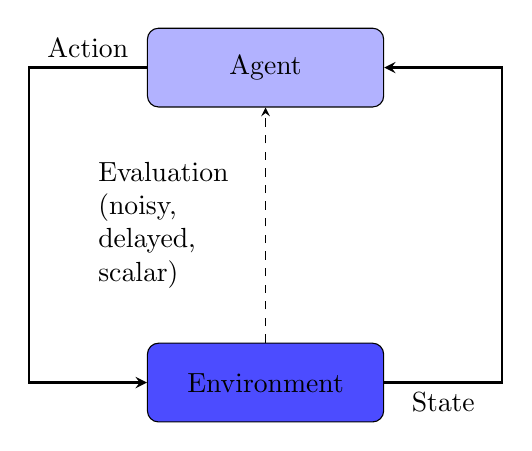
\begin{tikzpicture}
\tikzstyle{startstop} = [rectangle, rounded corners, minimum width=3cm, minimum height=1cm,text centered, draw=black, fill=blue!30]
\tikzstyle{io} = [rectangle, rounded corners, minimum width=3cm, minimum height=1cm,text centered, draw=black, fill=blue!70]
\tikzstyle{arrow} = [thick,->,>=stealth]
\tikzstyle{arrow2} = [dashed,->,>=stealth]
\node (start) [startstop] {Agent};
\node (in1) [io, below of=start, yshift=-3.0cm] {Environment};
\draw [arrow] (in1.east) -- node[anchor=north] {State} ++ (1.5cm,0) |- (start.east);
\draw [arrow] (start.west) -- node[anchor=south] {Action} ++ (-1.5cm,0) |- (in1.west);
\draw [arrow2] (in1.north) -- node[anchor=east, text width=2cm] {Evaluation (noisy, delayed, scalar)} (start.south);
\end{tikzpicture}
\end{center}
\caption{General framework}\label{rlflow}
\end{figure}

Crux: Agent work in close interaction with environment. It senses the state of the environment, take action and see how state is affected. Don't choose actions that are beneficial in the current state but actions that put you in a beneficial state in the future

\textbf{Assumption:} Environment gives some form of evaluation. This evaluation may be noisy and temporally delayed. In reality, all sensory input received from the surroundings is processed and some part of the brain interprets some of the sensory input as reward/punishment. Evaluation is assumed (defined) to be a scalar. This scalar is to be maximised over time.

\textbf{Not supervised learning: } In RL, there is very \textit{sparse} supervision and no target output. Since there is no error function given by the environment, trial-and-error is essential for estimating gradient.

\begin{figure}[!htbp]
\begin{center}
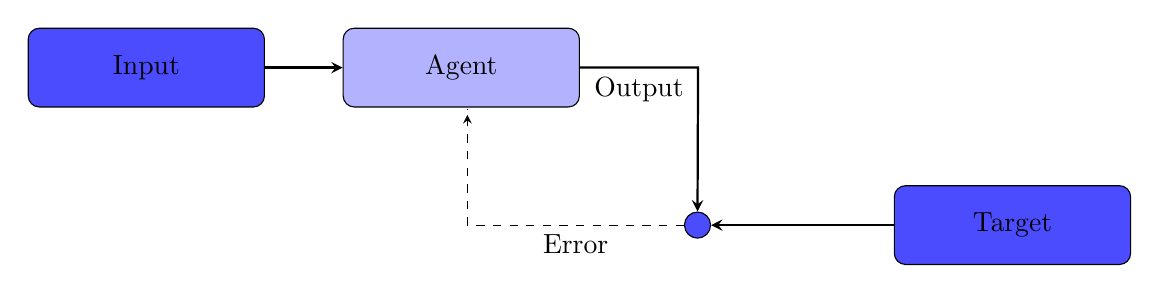
\begin{tikzpicture}
\tikzstyle{startstop} = [rectangle, rounded corners, minimum width=3cm, minimum height=1cm,text centered, draw=black, fill=blue!30]
\tikzstyle{io} = [rectangle, rounded corners, minimum width=3cm, minimum height=1cm,text centered, draw=black, fill=blue!70]
\tikzstyle{er} = [circle, text centered, draw=black, fill=blue!70]
\tikzstyle{arrow} = [thick,->,>=stealth]
\tikzstyle{arrow2} = [dashed,->,>=stealth]
\node (start) [startstop] {Agent};
\node (in1) [io, left of=start, xshift=-3.0cm] {Input};
\node (in2) [io, right of=start, xshift=6.0cm, yshift=-2cm] {Target};
\node (err) [er, right of=start, xshift=2.0cm, yshift=-2cm] {};
\draw [arrow] (in1.east) -- (start.west);
\draw [arrow] (start.east) -- node[anchor=north] {Output} ++ (1.5cm,0) -- (err.north);
\draw [arrow] (in2.west) -- (err.east);
\draw [arrow2] (err.west) -- node[anchor=north] {Error} ++ (-2.75cm,0) |- ++(0, 1.4cm);
\end{tikzpicture}
\end{center}
\caption{Supervised learning framework}\label{slflow}
\end{figure}

\textbf{Not unsupervised learning:} There is sparse supervision. Also, pattern discovery is not the primary goal in RL.

\textbf{Temporal difference learning:} The prediction of eventual outcome at time \textit{t+1} will be better than the prediction at time \textit{t}. Hence use the later prediction to adjust earlier prediction. TD learning seems to explain some neurotransmitter behaviour in the brain.

\textbf{Explore-Exploit dilemma:} Explore to find other/more profitable actions and exploit to act according to the best actions already made.

\section{Immediate Reinforcement Learning Problems}
In this category of problems, reward is obtained immediately after an action i.e. there is no time delay between action and reward. 

\textbf{Notation:} At time \textit{t}, an action $a_t$ results in reward $R_t$.

Notice that we do not mention a time/state dependent input. The agent here receives the same input at all time instants, i.e. it always plays the same one-step game.

The outcome may be stochastic. The same action can result in different rewards at different instances. Thus, the effect of different actions should be \textit{explored}. However, we are interested in eventually \textit{exploiting} the knowledge acquired.

The payoff is assumed to be obtained from a distribution that depends on the action chosen but does not change over multiple experiments\footnote{if X is RV with cdf C, then distribution can be sampled by returning $C^{-1}(uniform(0,1))$}. If the distributions were known, the optimal move would be to select the action with highest expected payoff. Thus, the problem here is to figure out the different distributions.

\textbf{Notation:} Associated with each action \textit{a} let the \textbf{true} expected payoff be $q_*(a)$

\subsection{Bandit problems}
\textbf{Notation:} \textit{One-armed bandit} is a slot machine where you put in a coin, pull a lever (arm) and get reward(mostly none hence the name bandit)

Multi-arm bandit is essentially this slot machine with multiple levers with different payoff distributions.

Solution of multi-arm bandit problem can involve:
\begin{enumerate}
\item Asymptotic correctness: There are not constraints but give a guarantee that eventually the agent selects the arm with the highest expected payoff.
\item Regret optimality\footnote{ E.g.: we design a sophisticated online algorithm that deals with various issues of uncertainty and decision making, and sell it to a client. Our algorithm runs for some time and incurs a certain loss. We would like to avoid the embarrassment that our client will come back to us and claim that in retrospect we could have incurred a much lower loss if we used his simple alternative policy $\pi$. The regret of our online algorithm is the difference between the loss of our algorithm and the loss using $\pi$.}: Suppose the agent expores the problem space and accumulates reward till time \textit{t}. The difference between this reward and the reward obtained if the optimal action was followed from the beginning is the \textit{regret}. Regret optimality aims to maximize the total reward obtained (even in the learning phase), i.e. we want to reach the maximum expected payoff quickly. It is an established result that regret grows/accumulates at least at rate $log(t)$.
\item Probably approximately correct (PAC) optimality: With a high probabilty (probably) the arm returned as result will give expected payoff close to optimal expected payoff (approximately correct). $(\epsilon, \delta)-PAC$ means that with probability $(1-\delta)$ the solution returned will be within $\epsilon$ of the optimal solution i.e. $Pr\{q(result) \geq q_{*}(a^*) - \epsilon\} \geq (1-\delta)$. $(\epsilon, \delta)-PAC$ optimality is smallest number of times the arms are sampled such that the agent can give the $(\epsilon, \delta)-PAC$ gurantee.
\end{enumerate}

1 is a question of correctness, 2 is a question of rate of convergence and 3 is a sample complexity question.

\subsection{Action-Value Methods}
\textbf{Notation:} $Q_t(a)$ is the \textit{estimated} expected payoff of an action i.e. an approximation of $q_*(a)$ the true expected payoff.

$Q_t(a) = \frac{\sum_{i=1}^t 1_{a_i=a}.R_i}{\sum_{i=1}^t 1_{a_i=a}}$

\begin{enumerate}
\item Greedy policy: action chosen = $\argmaxF_a Q_t(a)$ 
\item $\epsilon$-greedy: With probability $(1-\epsilon)$ be greedy and with probability $\epsilon$ explore (choose any random action)
\item softmax: $Pr\{a_{t+1}=a\} = \frac{e^{Q(a)/\beta}}{\sum_{b=1}^n e^{Q(b)/\beta}}$ where $\beta$ is a temperature parameter. High $\beta$ spreads probability (more random) over actions while low $\beta$ (cooler,calmer) gives peakier distribution.
\end{enumerate}

Asymptotic correctness of the $\epsilon$-greedy approach is ensured as exploration and exploitation are balanced. However, to ensure choice of only the optimal arm in the long run, $epsilon$ must be cooled down. Decreasing $\epsilon$ as 1/t is proposed but this converges to zero only asymptotically, so instead $\epsilon$ can be cooled in steps.

\subsection{Incremental Implementation}
To calculate $Q_t(a)$ without having to store the previous values,

$Q_t(a) = Q_{t-1}(a) + \frac{1_{a_t=a}}{n_a + 1_{a_t=a}}[R_t.1_{a_t=a} - Q_{t-1}(a)]$

This is an unbaised estimate of the mean payoff of action a. This converges if the reward is obtained from a stationary process. For non-stationary reward process, the update rule must be modified to give more weight to recent samples than long-past ones. Modified update rule:

$Q_t(a) = Q_{t-1}(a) + \alpha.1_{a_t=a}[R_t.1_{a_t=a} - Q_{t-1}(a)]$

where $\alpha$, step-size parameter, lies in (0,1]. When expanded, we see that the weight of reward $R_i$ is $\alpha(1-\alpha)^i$ which is exponentially decaying.

\textbf{Book notes}\\
Sometimes it is convenient to vary the step-size parameter from step to step. Let $\alpha_k(a)$ denote the step-size parameter used to process the reward received after the kth (k = $n_a + 1_{a_t=a}$) selection of action a. As we have noted, the choice $\alpha_k(a) = \frac{1}{k}$ results in the sample-average method, which is guaranteed to converge to the true action values by the law of large numbers. But of course convergence is not guaranteed for all choices of the sequence {α k (a)}. A well-known result in stochastic approximation theory gives us the conditions required to assure convergence with probability 1:

$\sum_{k=1}^\infty a_k = \infty$	and	$\sum_{k=1}^\infty a_k^2 < \infty$

The first condition is required to guarantee that the steps are large enough to eventually overcome any initial conditions or random fluctuations. The second condition guarantees that eventually the steps become small enough to assure convergence. Note that both convergence conditions are met for the sample-average case, $\alpha_k(a) = \frac{1}{k}$, but not for the case of constant step-size parameter, $\alpha_k(a) = \alpha$.

\section{Quick Links}
\begin{itemize}
\item \href{https://courses.cs.washington.edu/courses/cse590hk/01sp/Readings/tesauro95cacm.pdf}{Temporal difference learning and TD-Gammon}
%\item \href{}{}
\end{itemize}

\end{document}